\PassOptionsToPackage{table,xcdraw}{xcolor}

\documentclass[sigconf,review,anonymous]{acmart}
%\acmConference[ESEC/FSE 2021]{The 29th ACM Joint European Software Engineering Conference and Symposium on the Foundations of Software Engineering}{23 - 27 August, 2021}{Athens, Greece}

%\documentclass[sigconf,review, anonymous]{acmart}
%\documentclass[sigconf]{acmart}

\usepackage{booktabs}   %% For formal tables:
                        %% http://ctan.org/pkg/booktabs
\usepackage{subcaption} %% For complex figures with subfigures/subcaptions
                        %% http://ctan.org/pkg/subcaption
\usepackage{array}
\usepackage{amsmath,amsfonts}
\usepackage{algorithm}
\usepackage[noend]{algpseudocode}
%\usepackage{algorithmic}
\usepackage{graphicx}
\usepackage{textcomp}
\usepackage{float} 
\usepackage{listings}
\usepackage{xspace}
\usepackage{multirow}
\usepackage{amsthm}
\newtheorem{definition}{Definition}
\usepackage{balance}

\usepackage[skins]{tcolorbox}

\usepackage{xcolor,pifont}
\newcommand*\colourcheck[1]{%
	\expandafter\newcommand\csname #1check\endcsname{\textcolor{#1}{\ding{52}}}%
}
\colourcheck{blue}
\colourcheck{green}
\colourcheck{red}

\newtcolorbox{myframe}[2][]{%
  enhanced,colback=white,colframe=black,coltitle=black,
  sharp corners,
  toprule=1.0pt,
  rightrule=0.3pt,
  leftrule=0pt,
  bottomrule=0pt,
  fonttitle=\itshape\scshape\large,
  left=0pt,right=5pt,top=5pt,bottom=3pt,
  attach boxed title to top right={yshift=-0.3\baselineskip-0.4pt,xshift=-5mm},
  boxed title style={tile,size=minimal,left=0.2mm,right=0.5mm,
    colback=white,before upper=\strut},
  title=#2,#1
}

%\newcommand{\code}[1]{{\footnotesize\textsf{#1}}}

\newcommand{\tool}{\textsc{FixLocator}\xspace}

\newtheorem{Definition}{Definition}
\newtheorem{Claim}{Claim}
\newtheorem{Lemma}{Lemma}
\newtheorem{Theorem}{Theorem}

\newcolumntype{L}[1]{>{\raggedright\arraybackslash}p{#1}}
\newtheorem{observation}{Observation}
\newtheorem{property}{Property}
\newcommand{\code}[1]{{\footnotesize\texttt{#1}}}
\usepackage{amsthm}
 \definecolor{dkgreen}{rgb}{0,0.6,0}
\definecolor{gray}{rgb}{0.5,0.5,0.5}
\definecolor{mauve}{rgb}{0.58,0,0.82}
\lstset{frame=tb,
  language=Java,
  aboveskip=3mm,
  belowskip=3mm,
  showstringspaces=false,
  columns=flexible,
  basicstyle={\small\ttfamily},
  numbers=left,
  numberstyle=\tiny\color{gray},
  keywordstyle=\color{blue},
  commentstyle=\color{dkgreen},
  stringstyle=\color{mauve},
  breaklines=true,
  breakatwhitespace=true,
  tabsize=4
}



\begin{document}

%\title[{\tool}: Deep Fault Localization with Code Coverage Representation Learning]{{\tool}: Deep Fault Localization with Code Coverage Representation Learning}

\title[{\tool}: Fault Localization to Detect Fixing Locations]{{\tool}: Fault Localization to Detect Fixing Locations}


%%%---- AUTHORS BLOCK ------

%Yi Li:New Jersey Institute of Technology;Shaohua Wang:New Jersey
%Institute of Technology;Tien Nguyen:University of Texas at Dallas 

%\author{Yi Li}
%\affiliation{
%\institution{New Jersey Inst. of Technology, USA}
%}
%\email{yl622@njit.edu}
%\author{Shaohua Wang}
%\affiliation{
%\institution{New Jersey Inst. of Technology, USA}
%}
%\email{davidsw@njit.edu}
%\author{Tien N. Nguyen}
%\affiliation{
%\institution{University of Texas at Dallas, USA}
%}
%\email{tien.n.nguyen@utdallas.edu}


%\renewcommand{\shortauthors}{Li, Wang, and Nguyen}

\setcopyright{none}

\settopmatter{printacmref=false, printfolios=false}

\renewcommand\footnotetextcopyrightpermission[1]{} % removes footnote with conference information in first column


%(1) present information sorted in a way that a CNN can "see" patterns
%discriminating between faulty and non faulty statements more easily;

%(2) identify the actual crash statement to the network;

%(3) present more information to the deep neural network in the form of
%a summary of data dependences for each statement as well as source
%embedding; and

%(4) the suspiciousness of a statement is seen taking into account
%relationships to other statement, as opposed to a statement by itself”



%\input{sections/abstract}
\begin{abstract}
We present {\tool}, a DL-based fault localization approach supporting
the detection of buggy statements that need to be fixed accordingly at
the same time in one or multiple methods.
...
\end{abstract}


%\settopmatter{printacmref=true, printccs=true, printfolios=false}

%\begin{CCSXML}
%<ccs2012>
%<concept>
%<concept_id>10011007.10011006.10011073</concept_id>
%<concept_desc>Software and its engineering~Software maintenance tools</concept_desc>
%<concept_significance>500</concept_significance>
%</concept>
%</ccs2012>
%\end{CCSXML}

%\ccsdesc[500]{Software and its engineering~Software maintenance tools}

%\keywords{Deep Learning; Automated Program Repair; Context-based Code Transformation Learning}


\maketitle

\section{Introduction}

Detecting and fixing software defects is crucial for a software
development process. To reduce the efforts from developers in that
process, several {\em fault localization} (FL)
approaches~\cite{fl-survey} have been introduced to help localize the
source of the fault that needs to be fixed. The input of an FL model
is the execution of a test suite, in which some of the test cases are
passing or failing ones. Specifically, the key input is the {\em code
  coverage matrix} in which the rows and columns correspond to the
statements and test cases, respectively.  Each cell is assigned with
the value of 1 if the respective statement is executed in the
respective test case, and with the value of 0, otherwise.  An FL model
uses such information to identify the list of {\em suspicious lines of
  code} that are ranked based on their associated {\em suspiciousness
  scores}~\cite{fl-survey}. In recent advanced FL, several approaches
also support fault localization at method
level~\cite{DeepFL,icse21-fl}. 



%In the FL problem, given the execution of test cases, an FL tool
%identifies the set of {\em suspicious lines of code} with their
%associated suspiciousness scores~\cite{fl-survey}.  The key input of
%an FL tool is the {\em code coverage matrix} in which the rows and
%columns correspond to the source code statements and test cases,
%respectively.  Each cell is assigned with the value of 1 if the
%respective statement is executed in the respective test case, and with
%the value of 0, otherwise. In recent FL, several researchers also
%advocate for fault localization at method level~\cite{DeepFL}. FL at
%both levels are useful for developers.

The FL approaches can be broadly divided into the following
categories: {\em spectrum-based fault localization} (SBFL)
approaches~\cite{Ochiai,jones2001visualization,keller2017critical},
{\em mutation-based fault localization} (MBFL)
approaches~\cite{MUSE,papadakis2012using,Metallaxis}, and {\em machine
  learning (ML)} and {\em deep learning (DL)}~\cite{deepFL,icse21-fl}.
For SBFL approaches, the key idea is that a line covered more in the
failing test cases than in the passing ones is more suspicious than a
line executed more in the passing ones.
%
To improve SBFL, MBFL
approaches~\cite{MUSE,papadakis2012using,Metallaxis} enhance the code
coverage information by modifying a statement with mutation operators,
and then collecting code coverages when executing the mutated programs
with the test cases. The MBFL approaches apply suspiciousness score
formulas in the same manner as in SBFL approaches on the matrix for
each original statement and its mutated ones.
%
ML and DL-based FL approaches explore the code coverage matrix and
apply different neural network models for fault localization.


%{\em Spectrum-based fault localization} (SBFL)
%approaches~\cite{Ochiai,jones2001visualization,keller2017critical}
%take the recorded lines of code that were covered by each of the given
%test cases, and assigned each line of code a suspiciousness score
%based on the code coverage matrix. Despite using different
%formulas to compute that score, the idea is that a line covered more
%in the failing test cases than in the passing ones is more suspicious
%than a line executed more in the passing ones. A key drawback of those
%approaches is that the same score is given to the lines that have been
%executed in both failing and passing test cases. An example is the
%statements that are part of a block statement and executed at the
%same nested level. Another example is the conditions of the
%condition statements, e.g., \code{if}, \code{while}, \code{do},
%and \code{switch}. 

%To improve SBFL, {\em mutation-based fault localization} (MBFL)
%approaches~\cite{MUSE,papadakis2012using,Metallaxis}
%enhance the code coverage information by modifying a statement with
%mutation operators, and then collecting code coverages when executing
%the mutated programs with the test cases. They apply suspiciousness
%score formulas in the same manner as the spectrum-based FL approaches on
%the code coverage matrix for each original statement and its mutated
%ones. Despite the improvement, MBFL are not effective for the bugs
%that require the fixes that are more complex than a mutation
%(Section~\ref{motivexample}).

%{\em Machine learning (ML)} and {\em deep learning (DL)}
%have been used in fault localization. DeepFL~\cite{DeepFL}
%computes for each faulty method a vector with +200 scores in which
%each score is computed via a specific feature, e.g., a spectrum-based
%or mutation-based formula, or a code complexity metric. Despite its
%success, the accuracy of DeepFL is still limited. A reason could be
%that it uses various calculated scores from different formulas as a
%proxy to learn the suspiciousness of a faulty element, instead of
%fully exploiting the code coverage. Some formulas, such
%as the spectrum- and mutation-based formulas, inherently suffer from
%the issues as explained earlier with the statements covered by
%both failing and passing test cases.

Despite their successes, the state-of-the-art FL approaches are still
limited in locating all the fixing locations that need to be repaired
at the same time in the same fix. In real-world software development,
there are several bugs that require a fix to multiple lines of code in
one or multiple hunks in the same or different methods. {\em The
  fixing changes to those lines of code are dependent to one another
  and need to be made in the same fix for the program to pass the test
  cases}. For those bugs, applying the fixing change to one statement
at a time will not make the program pass the test case after the
change to one statement.
%
This capability to detect the fixing locations of the co-changes in a
fix for a bug (let us call it {\em Co-change Fixing Locations} ({\em
  CC Fix Locations})) is important for both the manual process of bug
fixing as well as the automated process of program repairing. For
manual process, such capability will save effort and time for
developers in locating all the buggy statements that need to be fixed
at the same time. For automated program repair (APR), such capability
will enable an APR model to correctly and completely make the changes
to fix a bug.

From the ranked list of suspicious statements returned from an
existing FL model, a naive approach to detect CC Fix Locations would
be to take the top $k$ statements in that list and to consider them as
to be fixed together. This naive solution might not be effective
because the mechanisms used in the state-of-the-art FL approaches have
never considered the co-change nature of those fixes. Our empirical
evaluation also confirmed that (Section~\ref{eval:sec}).


We propose {\tool}, a fault localization approach for buggy
statements/methods  ...

The contributions of this paper are listed as follows:

{\bf 1. Novel code coverage representation.} Our representation
enables fully exploiting test coverage matrix and taking advantage of
the CNN model in image recognition to localize~faults.

{\bf 2. {\tool}: Novel DL-based fault localization approach.} Test
case ordering and three sources of information allow treating FL as a
pattern recognition. Without ordering and statement dependencies, the
CNN model will not work~well.

{\bf 3. Extensive empirical evaluation.} We evaluated our model
against the most recent FL models at the statement and method levels,
in both within-project and cross-project settings, and for both C and
Java. Our replication package is available
at~\cite{FaultLocalization2021}.


\section{Motivating Example}
\label{motiv:section}

\subsection{Example and Observations}

\begin{figure}[t]
	\centering
	\lstset{
		numbers=left,
		numberstyle= \tiny,
		keywordstyle= \color{blue!70},
		commentstyle= \color{red!50!green!50!blue!50},
		frame=shadowbox,
		rulesepcolor= \color{red!20!green!20!blue!20} ,
		xleftmargin=1.5em,xrightmargin=0em, aboveskip=1em,
		framexleftmargin=1.5em,
                numbersep= 5pt,
		language=Java,
    basicstyle=\scriptsize\ttfamily,
    numberstyle=\scriptsize\ttfamily,
    emphstyle=\bfseries,
                moredelim=**[is][\color{red}]{@}{@},
		escapeinside= {(*@}{@*)}
	}
	\begin{lstlisting}[]
public void toSource(final CodeBuilder cb, int inputSeqNum, Node root) {
	......
(*@{\color{red}{-	String code = toSource(root, sourceMap);}@*)
(*@{\color{cyan}{+	String code = toSource(root, sourceMap, inputSeqNum == 0);}@*)
	if (!code.isEmpty()) {
		cb.append(code);
	}
	......
}
//--------------------------------------------------------------------------
(*@@Override@*)
String toSource(Node n) {
 initCompilerOptionsIfTesting();
(*@{\color{red}{-	return toSource(n, null);}@*)
(*@{\color{cyan}{+ 	return toSource(n, null, true);}@*)
}
//--------------------------------------------------------------------------
(*@{\color{red}{- private String toSource(Node n, SourceMap sourceMap) {}@*)
(*@{\color{cyan}{+ private String toSource(Node n, SourceMap sourceMap, boolean firstOutput) {}@*)
	......
  builder.setSourceMapDetailLevel(options.sourceMapDetailLevel);
(*@{\color{red}{-   builder.setTagAsStrict(}@*)
(*@{\color{cyan}{+   builder.setTagAsStrict(firstOutput}@*) && 
		options.getLanguageOut(a) == LanguageMode.ECMASCRIPT5_STRICT);
  builder.setLineLengthThreshold(options.lineLengthThreshold);
	......	
}	
	\end{lstlisting}
        \vspace{-15pt}
        %        \caption{A Multi-statement/Multi-method Bug Fix}
        \caption{Co-Change Fixing Locations for a Fault}
        \vspace{-6pt}
        \label{fig:motiv}
\end{figure}

Let us start with a real-world example on the bug fixes that
require multiple changes to multiple statements in different methods.
Figure~\ref{fig:motiv} shows a bug in Defects4J dataset. The bug
occurred when the method call to \code{setTagAsStrict} did not
consider the first output in its arguments. Therefore, for fixing, a
developer adds a new argument in the method \code{toSource} at line
19, and uses that argument in the method call \code{setTagAsStrict
  (firstOutput,...)} at line 23. Because the method \code{toSource} at
line 19 was changed, the two callers at line 3 of the method
\code{toSource} (line 1) and at line 14 of the method \code{toSource}
(line 12) need to be changed accordingly.

%This is a bug from Defects4J data that has three methods need to be fixed at the same time. The bug is caused by doing the method call $setTagAsStrict$ without checking if it is the first output. To fix this bug, firstly, for the method C, we need to add one more parameter $firstOutput$ for the method call $setTagAsStrict$. Then, for the method A and B, because they call the method C or override the method C, when adding a new parameter in the method C, they all need to do the same thing. We need to add $inputSeqNum == 0$ in method A and add $true$ in method B when calling the method C.

%In this bug, there are multiple statements that need to be fixed and they located in three different methods. Also, when analyzing the co-change information, the method A and method C have been fixed together before in the commit history. 


\begin{figure*}[t]
	\centering
	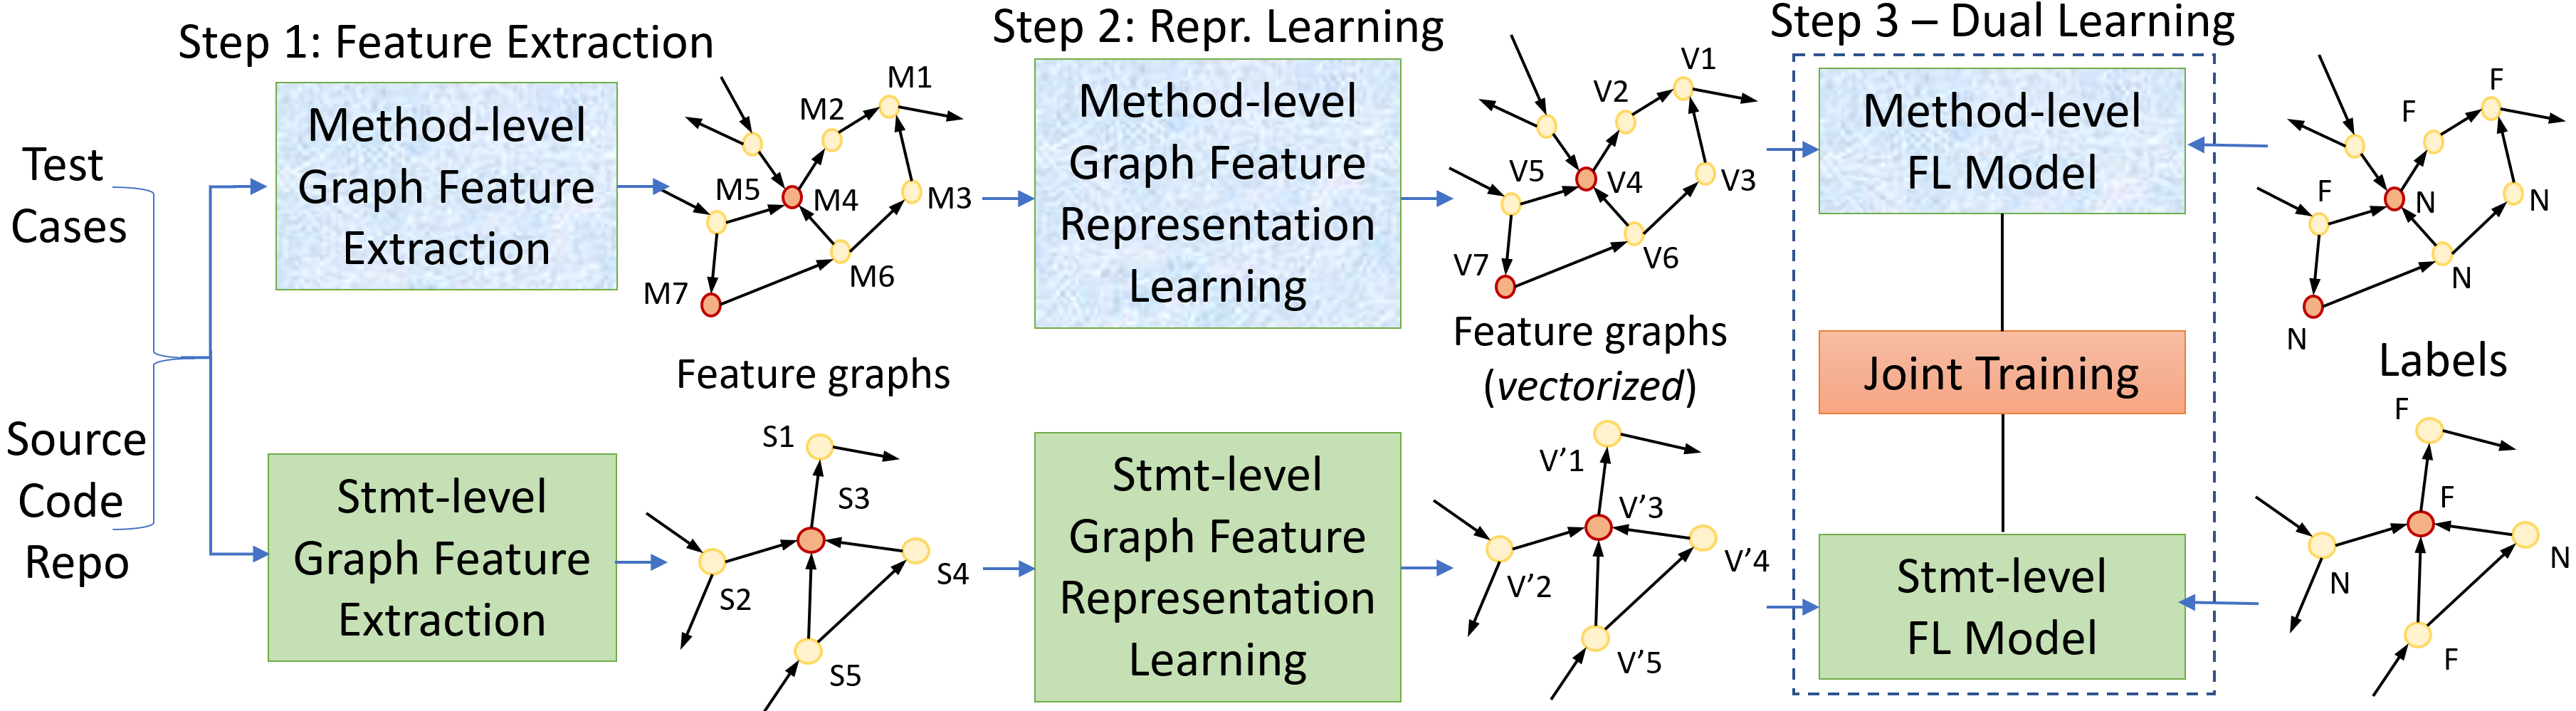
\includegraphics[width=5.45in]{graphs/overview-training.png}
        \vspace{-8pt}
	\caption{{\tool}: Training Process}
        \label{train-overview}
\end{figure*}

\noindent {\bf Observation 1. [Co-Change Fixing Locations]} As seen in
this example, the changes to fix this bug involve multiple faulty
statements that are dependent on one another. Fixing only one of the
faulty statements will not make the program pass the previously
failing test(s). For an APR model to work, an FL tool needs to point
out all of those faulty statements to be changed in the same fix. For
effective manually fixing by developers, an FL tool also needs point
out all faulty statements to be fixed at once. Otherwise, (s)he must
find the missing locations or waste time on incorrect ones.

\noindent {\bf Observation 2. [Multiple Faulty Methods]} As seen, this
bug requires the changes to three different methods at the same time.
It is important for an FL tool to connect and identify these multiple
faulty statements in potentially different methods.

%Traditional FL approaches~\cite{zhang-fse09,ICICA-10} using program
%analysis (PA), e.g., execution flow analysis, could identify all of
%those statements in the same fix due to their caller/callee
%relations.

Traditional FL approaches~\cite{zhang-fse09,ICICA-10} using program
analysis (PA), e.g., execution flow analysis, are restricted to
specific PA techniques, thus, not general to locate all types of CC
fixing locations.
%could identify all of those statements in the same fix due to their
%caller/callee relations.
Spectrum-based~\cite{jones2005empirical,abreu2006evaluation},
mutation-based~\cite{MUSE,papadakis2012using,Metallaxis}),
statistic-based~\cite{liblit-pldi05}, and machine learning (ML)-based
FL approaches~\cite{DeepFL,icse21-fl} could implicitly learn the
program dependencies for FL purpose. However, despite their successes,
the non-PA FL approaches {\em do not support the detection of multiple
  locations that need to be changed in the same fix for a bug, i.e.,
  Co-Change (CC) Fixing Locations}.
%
The spectrum-based and ML-based FL models return a ranked list of
suspicious statements according to the corresponding suspiciousness
scores. In this example, the lines 3, 14, 18, 22, and the other lines
({\em e.g.}, 5, 13, 21 and 25) are executed in the same passing or
failing test cases, thus~assigned with the same scores by
spectrum- and mutation-based FL approaches. A user would not be
informed on what lines need to be fixed together. Those non-PA,
especially ML-based FL approaches, do not have a mechanism to detect CC
fixing locations.

In this work, we aim to advance the level of deep learning (DL)-based
FL approaches to detect CC fixing locations. However, it is not
trivial. A solution of assuming the top-$k$ suspicious statements from
a FL tool as CC fixing locations does not work because even being the
most suspicious, those statements might not need to be changed in the
same fix. In this example, all of the above lines with the same
suspiciousness scores would confuse a fixer.

Moreover, another naive solution would be to use a method-level FL
tool to detect multiple faulty methods first and then use a
statement-level FL tool to detect the statements within each faulty
method. As we will show in our experiment, the inaccuracy of the first
phase of detecting faulty methods will have a confounding effect in
the overall performance in detecting CC fixing statements.




%\section*{Acknowledgments}
%This work was supported in part by the US National Science Foundation
%(NSF) grants CCF-1723215, CCF-1723432, TWC-1723198, CCF-1518897, and
%CNS-1513263.

\newpage

\balance

%\bibliographystyle{plain}
%\bibliographystyle{ACM-Reference-Format}
\bibliographystyle{ACM-Reference-Format}

\bibliography{References}

\end{document}
